\documentclass{standalone}

\usepackage{tikz}
\usepackage{xcolor}
\definecolor{primary}{HTML}{003262} % berkeley blue
\definecolor{secondary}{HTML}{FDB515} % cal gold
\definecolor{founder}{HTML}{3B7EA1}
\definecolor{medalist}{HTML}{C4820E}
\definecolor{goldengate}{HTML}{ED4E33}
\definecolor{ion}{HTML}{CFDD45}

\begin{document}
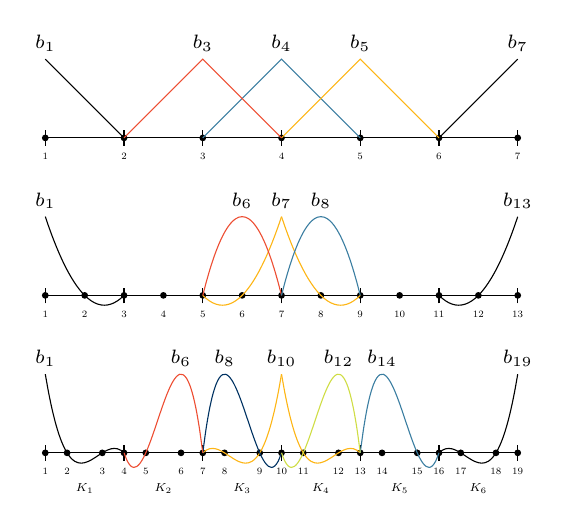
\begin{tikzpicture}
	\def\gap{.15cm}
	\scriptsize
	\draw (0,-.1) grid (6,.1); 
	% \foreach \i in {1,...,6}{
	% 	\node[scale=.75] at (\i-.5,-.35) {$K_{\i}$}; 
	% }
	\foreach \i in {1,...,7}{
		\filldraw (\i-1,0) circle[radius=1pt] node[below=\gap, scale=.5] {\i}; 
	}

	\draw (0,1) node[above] {$b_1$} -- (1,0); 
	\draw (5,0) -- (6,1) node[above] {$b_7$}; 
	\draw[founder] (2,0) -- (3,1) node[above, black] {$b_4$} -- (4,0); 
	\draw[secondary] (3,0) -- (4,1) node[above, black] {$b_5$} -- (5,0); 
	\draw[goldengate] (1,0) -- (2,1) node[above, black] {$b_3$} -- (3,0); 

	\begin{scope}[yshift=-2cm]
		\draw (0,-.1) grid (6,.1); 
		% \foreach \i in {1,...,6}{
		% 	\node[scale=.5] at (\i-.5,-.35) {$K_{\i}$}; 
		% }
		\foreach[evaluate=\i as \x using (\i-1)*6/12] \i in {1,...,13}{
			\filldraw (\x,0) circle[radius=1pt] node[below=\gap, scale=.5] {\i}; 
		}
		% left boundary 
		\draw[domain=0:1, smooth] plot(\x,{(\x-1)*(\x-.5)*2}); 
		\node at (0,1.2) {$b_1$}; 

		% right boundary 
		\draw[domain=0:1, smooth, xshift=5cm] plot(\x,{\x*(\x-.5)*2}); 
		\node at (6,1.2) {$b_{13}$}; 

		% interior shape 
		\draw[domain=0:1, smooth, xshift=2cm, secondary] plot(\x,{\x*(\x-.5)*2}); 		
		\draw[domain=0:1, smooth, xshift=3cm, secondary] plot(\x,{(\x-1)*(\x-.5)*2}); 
		\node at (3,1.2) {$b_{7}$}; 

		% interior bubble 
		\draw[domain=0:1, smooth, xshift=2cm, goldengate] plot(\x,{\x*(1-\x)*4}); 
		\node at (2.5,1.2) {$b_{6}$}; 
		\draw[domain=0:1, smooth, xshift=3cm, founder] plot(\x,{\x*(1-\x)*4}); 
		\node at (3.5,1.2) {$b_{8}$}; 
	\end{scope}

	\begin{scope}[yshift=-4cm]
		\draw (0,-.1) grid (6,.1); 
		\foreach \e in {0,...,5}{
			\foreach \i [count=\j from 3*\e+1] in {0,.276393,.723606}{
				\filldraw (\e+\i,0) circle[radius=1pt] node[below=\gap, scale=.5] {\j}; 
			}
		}
		\filldraw (6,0) circle[radius=1pt] node[below=\gap, scale=.5] {19}; 

		% left boundary 
		\draw[domain=0:1, smooth] plot(\x, {-5*\x^3 + 10*\x^2 - 6*\x + 1}); 
		\node at (0,1.2) {$b_1$}; 
		% right boundary 
		\draw[domain=0:1, smooth, xshift=5cm] plot(\x, {5*\x^3 - 5*\x^2 + 1*\x}); 
		\node at (6,1.2) {$b_{19}$}; 
		
		% interior shape 
		\draw[domain=0:1, smooth, xshift=2cm, secondary] plot(\x, {5*\x^3 - 5*\x^2 + 1*\x}); 
		\draw[domain=0:1, smooth, xshift=3cm, secondary] plot(\x, {-5*\x^3 + 10*\x^2 - 6*\x + 1}); 
		\node at (3,1.2) {$b_{10}$}; 

		% bubbles
		\draw[domain=0:1, smooth, xshift=2cm, primary] plot(\x, {11.1803399*\x^3 - 19.2705098*\x^2 + 8.09016994*\x}); 
		\node at (2.276393,1.2) {$b_8$}; 

		\draw[domain=0:1, smooth, xshift=1cm, goldengate] plot(\x, {-11.1803399*\x^3 + 14.2705098*\x^2 - 3.09016994*\x}); 
		\node at (1.723606,1.2) {$b_6$}; 

		\draw[domain=0:1, smooth, xshift=4cm, founder] plot(\x, {11.1803399*\x^3 - 19.2705098*\x^2 + 8.09016994*\x}); 
		\node at (3.723606,1.2) {$b_{12}$}; 

		\draw[domain=0:1, smooth, xshift=3cm, ion] plot(\x, {-11.1803399*\x^3 + 14.2705098*\x^2 - 3.09016994*\x}); 
		\node at (4.276393,1.2) {$b_{14}$}; 

		\foreach \i in {1,...,6}{
			\node[scale=.6] at (\i-.5,-.45) {$K_{\i}$}; 
		}
	\end{scope}
\end{tikzpicture}
\end{document}